\section{Projections of differential Higgs boson production cross sections and their interpretation}

\emph{%
This section covers the projection of the results from Sections~\ref{sec:diffxs} and \ref{sec:interpretation} to the integrated luminosity to be obtained by the High-Luminosity Large Hadron Collider -- $3000\fbinv$.
% 
First a short introduction on the High-Luminosity LHC is given, followed by a short discussion of the treatment of systematic uncertainties, and concluded with the projections of the $\pth$ spectrum and its interpretation.
% 
Section~\ref{sec:projection-results}, treating the projections, closely follows the original text from Ref.~\cite{CMS:2018qgz}.
}


\subsection{The High-Luminosity LHC}

The LHC and its detectors operate under a harsh radiation environment, and as such its equipment has a limited lifetime.
% 
In preparation for the upcoming data-taking period, which starts in 2021 and is known in the community as `Run 3', already significant upgrades to the ATLAS and CMS detectors have taken place.
% 
However, a number of key components of the LHC and its detectors will reach the end of their lifetime in the 2020s~\cite{Apollinari:2017cqg}.
% 
Moreover, after Run 3 it is of limited use to run at the current values of instantaneous luminosity: Without any hardware upgrade, it would take over 10 years to halve the statistical component of the uncertainty of a given measurement~\cite{Apollinari:2017cqg} at the end of Run 3.
% 
In preparation for the needed hardware replacement, already in 2011 the High-Luminosity Large Hadron Collider project (HL-LHC) was initiated, aiming to exploit the LHC to its fullest extent.
% 
Among the most difficult technical challenges are innovative $11$-$12\,$T superconducting magnets, highly compact superconducting cavities for beam rotation with ultra-precise phase control, new technology for beam collimation, and high-power superconducting links with almost zero energy dissipation~\cite{Apollinari:2017cqg}.
% 
The project comprises hardware upgrades, many of which require innovations to overcome serious technical challenges, and projected physics results for the LHC and all of its detectors.
% 
The project was formally approved in 2015, and the required research, development and implementation is expected to take at least 10 years.
% 
Overall, the HL-LHC is expected to take about $3000\fbinv$ of data over about 12 years of operation, a factor 10 increase with respect to the data available at the end of Run 3.


\subsection{Scenarios for the systematic uncertainties at \texorpdfstring{$3000\fbinv$}{3000 fb-1}}

By construction, given $N$ times the current amount of data, the statistical component of the uncertainty of any given measurement is expected to improve by a factor of $1/\sqrt{N}$.
% 
The systematic component is less obvious: some are estimated using data, and it can be reasonably assumed that they will improve for HL-LHC; for others, the magnitude will depend greatly on the implementation of the hardware upgrades.
% 
Meaningfully projecting current results to $3000\fbinv$ requires some assumptions on the systematic uncertainties.
% 
In the context of Higgs boson physics, CMS and ATLAS have jointly defined \textit{scenarios} for systematic uncertainties~\cite{s1s2talk}:
% 
\begin{itemize}
\item \textbf{Scenario 1 (S1):} Systematic uncertainties are kept constant. Essentially the performance of the detector is in this case assumed to unchanging;
% 
\item \textbf{Scenario 2 (S2):} Per systematic uncertainty, a decision is made on its scaling behavior given more luminosity. The recommendations for systematic uncertainties can be found in more detail in Ref.~\cite{CMS:2018qgz}.
% 
\item \textbf{Statistical uncertainty only:} It is assumed that the systematic uncertainties vanish entirely.
\end{itemize}
% 
Scenario 1 can be considered a pessimistic scenario, as it assumes no improvement of the detector at all.
% 
The scenario considering only statistical uncertainties is the most optimistic scenario; and scenario 2, the most `realistic' one, lies somewhere in between S1 and S2.
% 
For the projections of the interpretations of differential cross sections only S1 and S2 will be considered.



\subsection{Projections for the  \texorpdfstring{$\pth$}{pT(H)} spectrum and its interpretations}
\label{sec:projection-results}

The projections are carried out using the same analysis framework as used for the results in Sections~\ref{sec:diffxs} and \ref{sec:interpretation}.
% 
Of all the differential observables, only the $\pth$ spectrum is currently projected, as it is the only one which is interpreted.
% 
The cross sections in all bins are determined from a simultaneous maximum likelihood fit as described in section~\ref{sec:stat}, including the effects of bin-to-bin migrations.
% 
The projections all concern an \emph{expected} result given a larger dataset.
% 
The amount of expected events is scaled up by a factor of $3000 / 35.9$, i.e. the expected integrated luminosity at the end of HL-LHC over the integrated luminosity of the current results.


% ____________________________________________________________________________
\subsubsection{The differential cross section for \texorpdfstring{$\pth$}{pTH}}

The projection of the differential cross section for the $\pth$ spectrum is shown in Fig.~\ref{fig:proj_pth}, for both S1 and S2.
% 
The relative uncertainties for all scenarios are given in Tables~\ref{tab:proj_pth_unc_scen1}--\ref{tab:proj_pth_unc_statonly}.
% and \ref{tab:proj_pth_unc_scen2}.
% 
With respect to the uncertainties at the current integrated luminosity of 35.9\fbinv, the uncertainties at 3000\fbinv in the higher $\pth$ region are about a factor of ten smaller. This is expected, as the uncertainties in this region remain statistically dominated.
% 
The uncertainties in the lower $\pth$ region are no longer statistically dominated however, as can been seen by comparing Table~\ref{tab:proj_pth_unc_scen1} with Table~\ref{tab:proj_pth_unc_scen2}, where the reduced systematic uncertainties in S2 yield a reduction in the total uncertainty of up to 25\% compared to S1.
% 
As expected, the systematic uncertainties in S2 lie in between those of S1 and the statistical-uncertainty-only scenario.


\begin{table}[htb]
\footnotesize
\begin{center}
\begin{tabular}{|l|c|c|c|c|c|c|c|c|c|}
\hline
$\pth$       & 0-15    &  15-30   &  30-45    &  45-80   &  80-120  &  120-200  &  200-350  &  350-600  &  600-$\infty$  \\
\hline
$\hgg$       & 7.16\%  &  6.82\%  &  7.13\%   &  6.94\%  &  7.05\%  &  6.65\%   &  7.09\%   &  9.87\%   &  32.55\%  \\
\hline
$\hzz$       & 6.21\%  &  5.66\%  &  \multicolumn{2}{c|}{5.02\%}  &  \multicolumn{2}{c|}{5.55\%}  &  \multicolumn{3}{c|}{9.56\%} \\
\hline
$\hbb$       & \multicolumn{7}{c|}{\textit{None}}                                                       &  38.22\%  &  37.11\%  \\
\hline
Combination  & 4.70\%  &  4.36\%  &  5.04\%   &  4.66\%  &  4.84\%  &  4.73\%   &  5.23\%   &  8.53\%   &  25.45\%  \\
\hline
\end{tabular}
\end{center}
\caption{
    Relative uncertainties on the projected $\pth$ spectrum under S1 at $3000\fbinv$.
    }
\label{tab:proj_pth_unc_scen1}
\end{table}

\begin{table}[htb]
\footnotesize
\begin{center}
\begin{tabular}{|l|c|c|c|c|c|c|c|c|c|}
\hline
$\pth$       & 0-15    &  15-30   &  30-45    &  45-80   &  80-120  &  120-200  &  200-350  &  350-600  &  600-$\infty$  \\
\hline
$\hgg$       &  5.12\%  &   4.55\%  &  5.10\%   &   4.78\%   &   4.94\%   &   4.52\%   &  5.10\%   &  8.57\%   &   32.24\%    \\
\hline
$\hzz$       &  5.36\%  &   4.80\%  &  \multicolumn{2}{c|}{4.06\%}   &   \multicolumn{2}{c|}{4.71\%}   &   \multicolumn{3}{c|}{9.10\%}  \\
\hline
$\hbb$       &  \multicolumn{7}{c|}{\textit{None}}                                                             &  31.41\%  &   36.81\%    \\
\hline
Combination  &  3.72\%  &   3.26\%  &  4.22\%   &   3.75\%   &   3.97\%   &   3.83\%   &  4.37\%   &  8.04\%   &   24.54\%    \\
\hline
\end{tabular}
\end{center}
\caption{
    Relative uncertainties on the projected $\pth$ spectrum under S2 (with YR18 systematic uncertainties) at $3000\fbinv$.
    }
\label{tab:proj_pth_unc_scen2}
\end{table}


\begin{table}[ht]
\footnotesize
\begin{center}
\begin{tabular}{|l|c|c|c|c|c|c|c|c|c|}
\hline
$\pth$       & 0-15    &  15-30   &  30-45    &  45-80   &  80-120  &  120-200  &  200-350  &  350-600  &  600-$\infty$  \\
\hline
$\hgg$       &  4.06\%  &  3.24\%  &  4.02\%  &  3.55\%  &  3.77\%  &  3.33\%   &  4.07\%  &  7.99\%   &  32.09\%    \\
\hline
$\hzz$       &  4.19\%  &  3.91\%  &  \multicolumn{2}{c|}{3.01\%}  &  \multicolumn{2}{c|}{3.88\%} &  \multicolumn{3}{c|}{8.79\%}  \\
\hline
$\hbb$       &  \multicolumn{7}{c|}{\textit{None}}                                                   &  25.63\%  &  30.59\%    \\
\hline
Combination  &  2.92\%  &  2.50\%  &  3.67\%  &  3.11\%  &  3.36\%  &  3.20\%   &  3.79\%  &  7.61\%   &  22.25\%    \\
\hline
\end{tabular}
\end{center}
\caption{
    Relative uncertainties on the projected $\pth$ spectrum  at $3000\fbinv$ assuming vanishing systematic uncertainties.
    }
\label{tab:proj_pth_unc_statonly}
\end{table}


\begin{figure}[hbtp]
  \begin{center}
    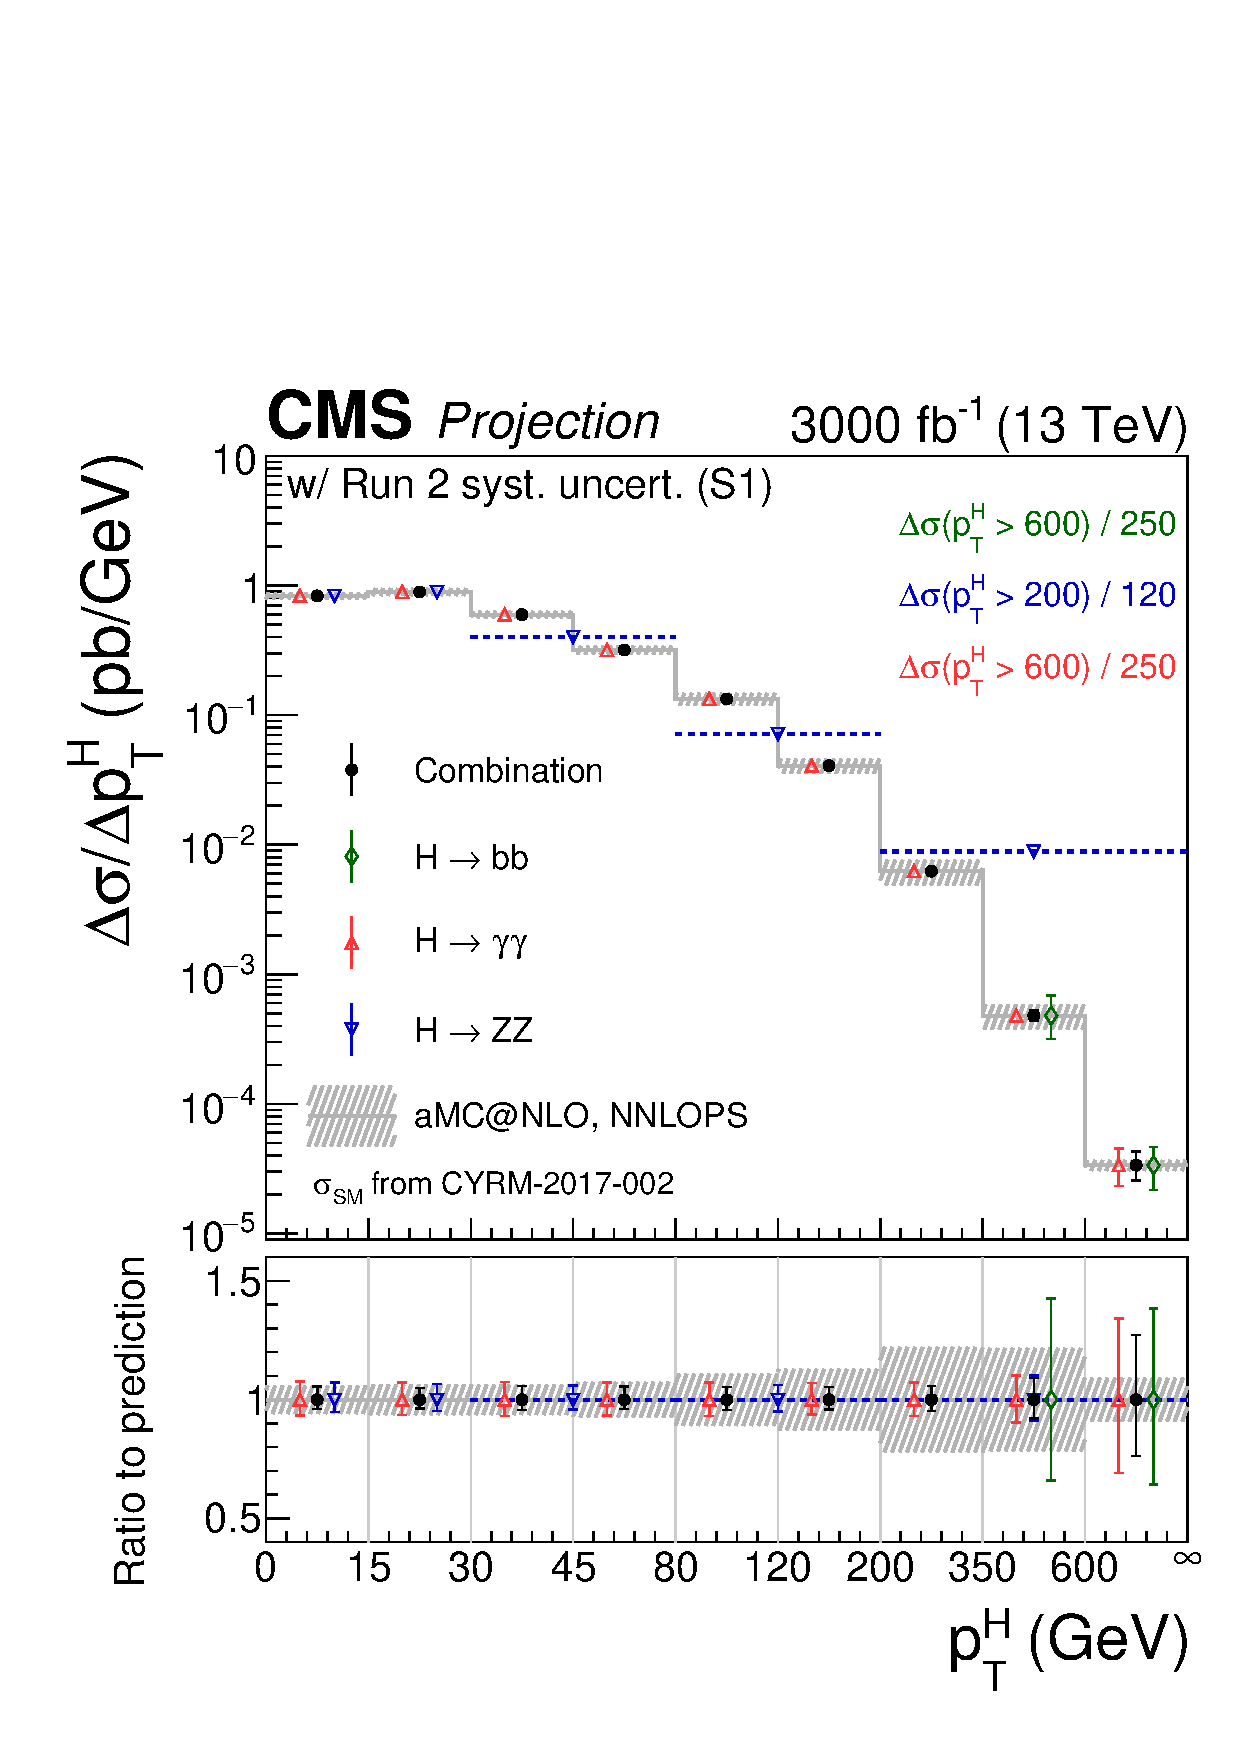
\includegraphics[width=0.49\linewidth]{img/projections/projectionspectra_pth_smH.pdf}
    % \includegraphics[width=0.49\linewidth]{img/projections/projectionspectra_pth_smH_statonly.pdf}
    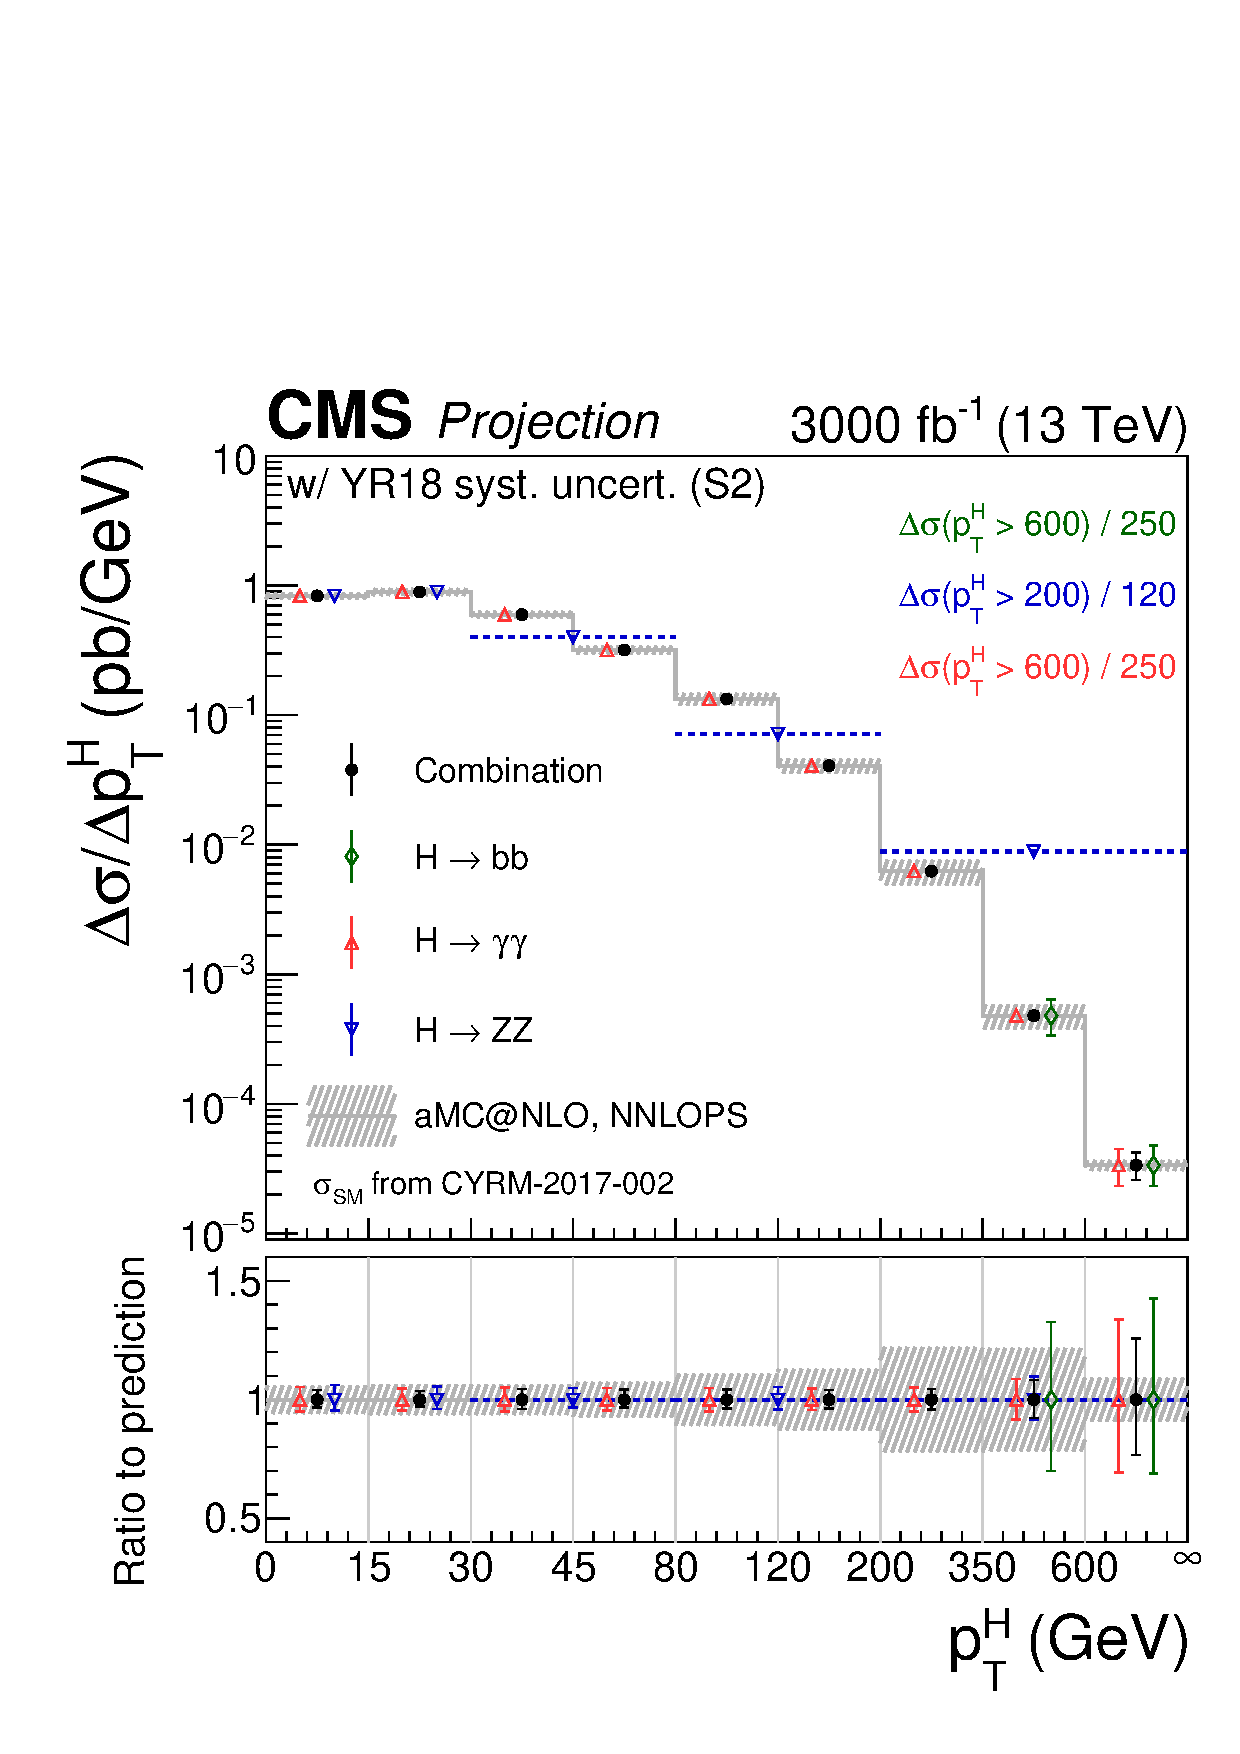
\includegraphics[width=0.49\linewidth]{img/projections/projectionspectra_pth_smH_scenario2.pdf}
    \caption{
        Projected differential cross section for the $\pth$ spectrum at an integrated luminosity of 3000\fbinv, under S1 (left) and S2 (right).
        }
    \label{fig:proj_pth}
  \end{center}
\end{figure}


% ____________________________________________________________________________
\subsubsection{Constraining Higgs coupling modifiers using the \texorpdfstring{$\pth$}{pTH} spectrum}

The $\pth$ spectrum is interpreted in terms of the same two theoretical models described in Section~\ref{sec:interpretation}.
% 
The results of the fits of $\kappab$/$\kappac$ and $\kappat$/$\cg$ are shown in Fig.~\ref{fig:proj_kbkc} and Fig.~\ref{fig:proj_ktcg}, respectively.
% 
The interpretation in terms of simultaneous variations of $\kappat$ and $\kappab$ are omitted.
% 
The theoretical uncertainties on the $\pth$ predictions, described in Section~\ref{sec:interpretation-systematics}, are included in the systematic uncertainties, and are not reduced with integrated luminosity.
% 
For this reason, the relative difference between S1 and S2 is expected not to be as pronounced as in the case of the differential $\pth$ combination.


\begin{figure}[hbtp]
  \begin{center}
    \ifbool{draftmode}{
        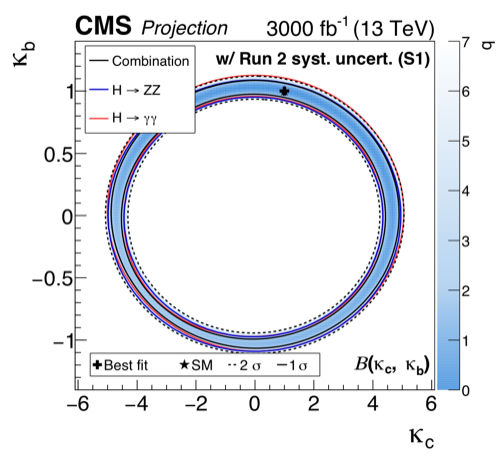
\includegraphics[width=0.49\linewidth]{img/projections/projection_kbkc_plot_couplingdependentBRs.png}
        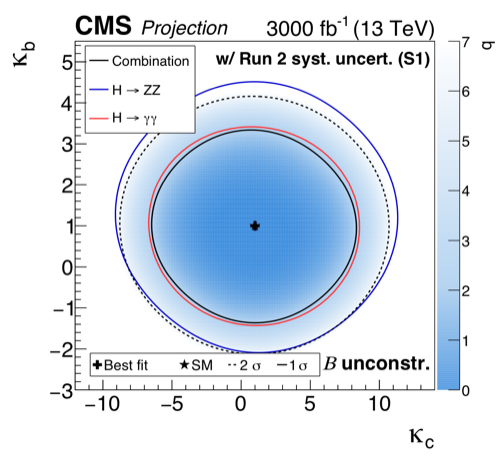
\includegraphics[width=0.49\linewidth]{img/projections/projection_kbkc_plot_floatingBRs.png}
        % 
        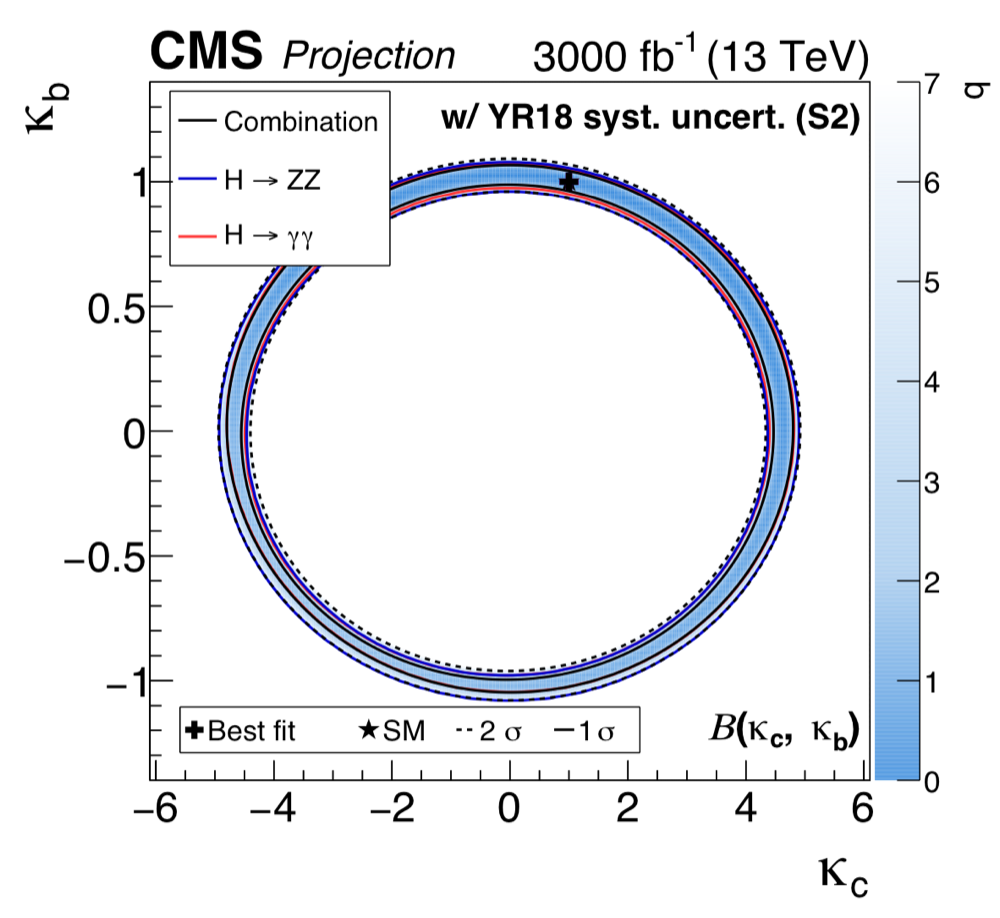
\includegraphics[width=0.49\linewidth]{img/projections/projection_kbkc_plot_couplingdependentBRs_scenario2.png}
        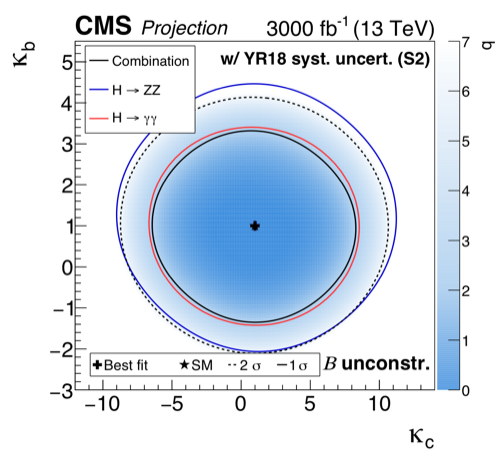
\includegraphics[width=0.49\linewidth]{img/projections/projection_kbkc_plot_floatingBRs_scenario2.png}
        }{
        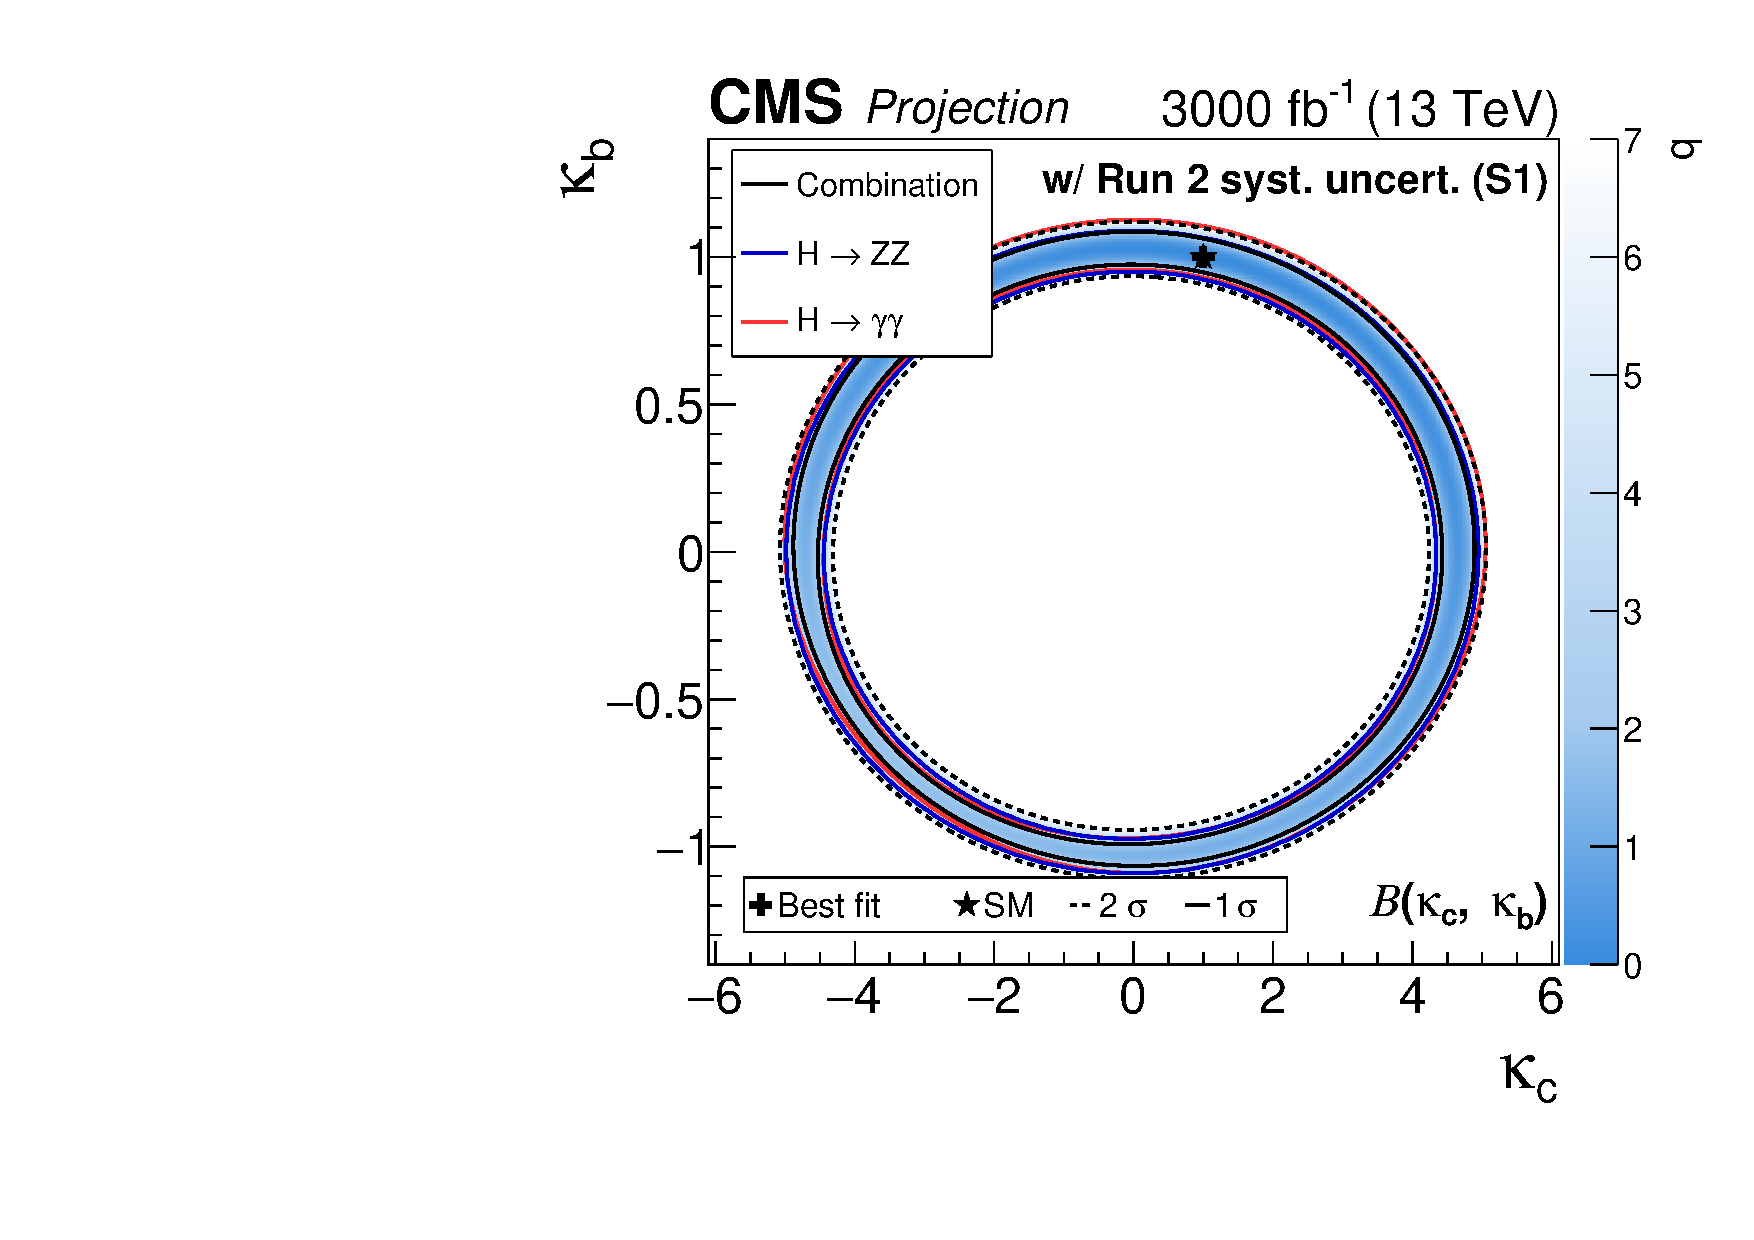
\includegraphics[width=0.49\linewidth]{img/projections/projection_kbkc_plot_couplingdependentBRs.pdf}
        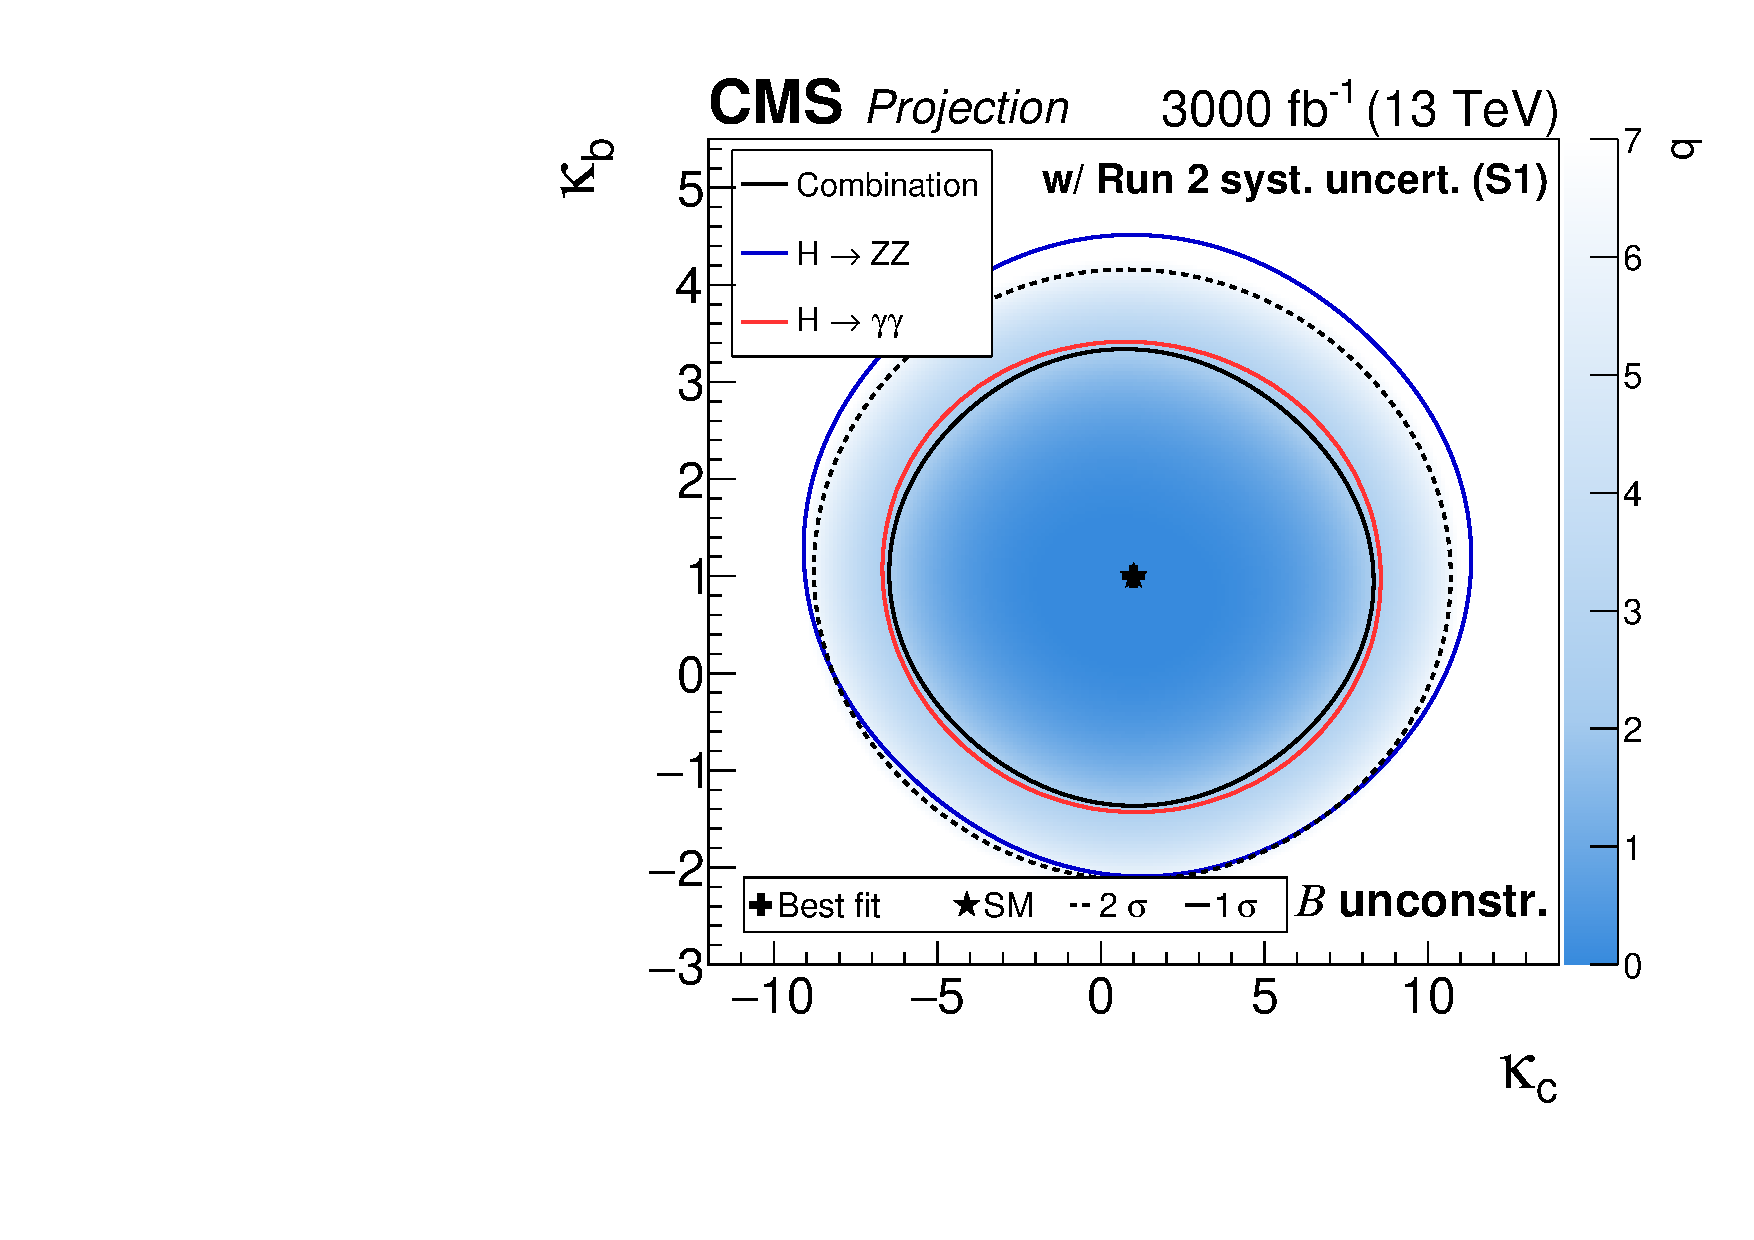
\includegraphics[width=0.49\linewidth]{img/projections/projection_kbkc_plot_floatingBRs.pdf}
        % 
        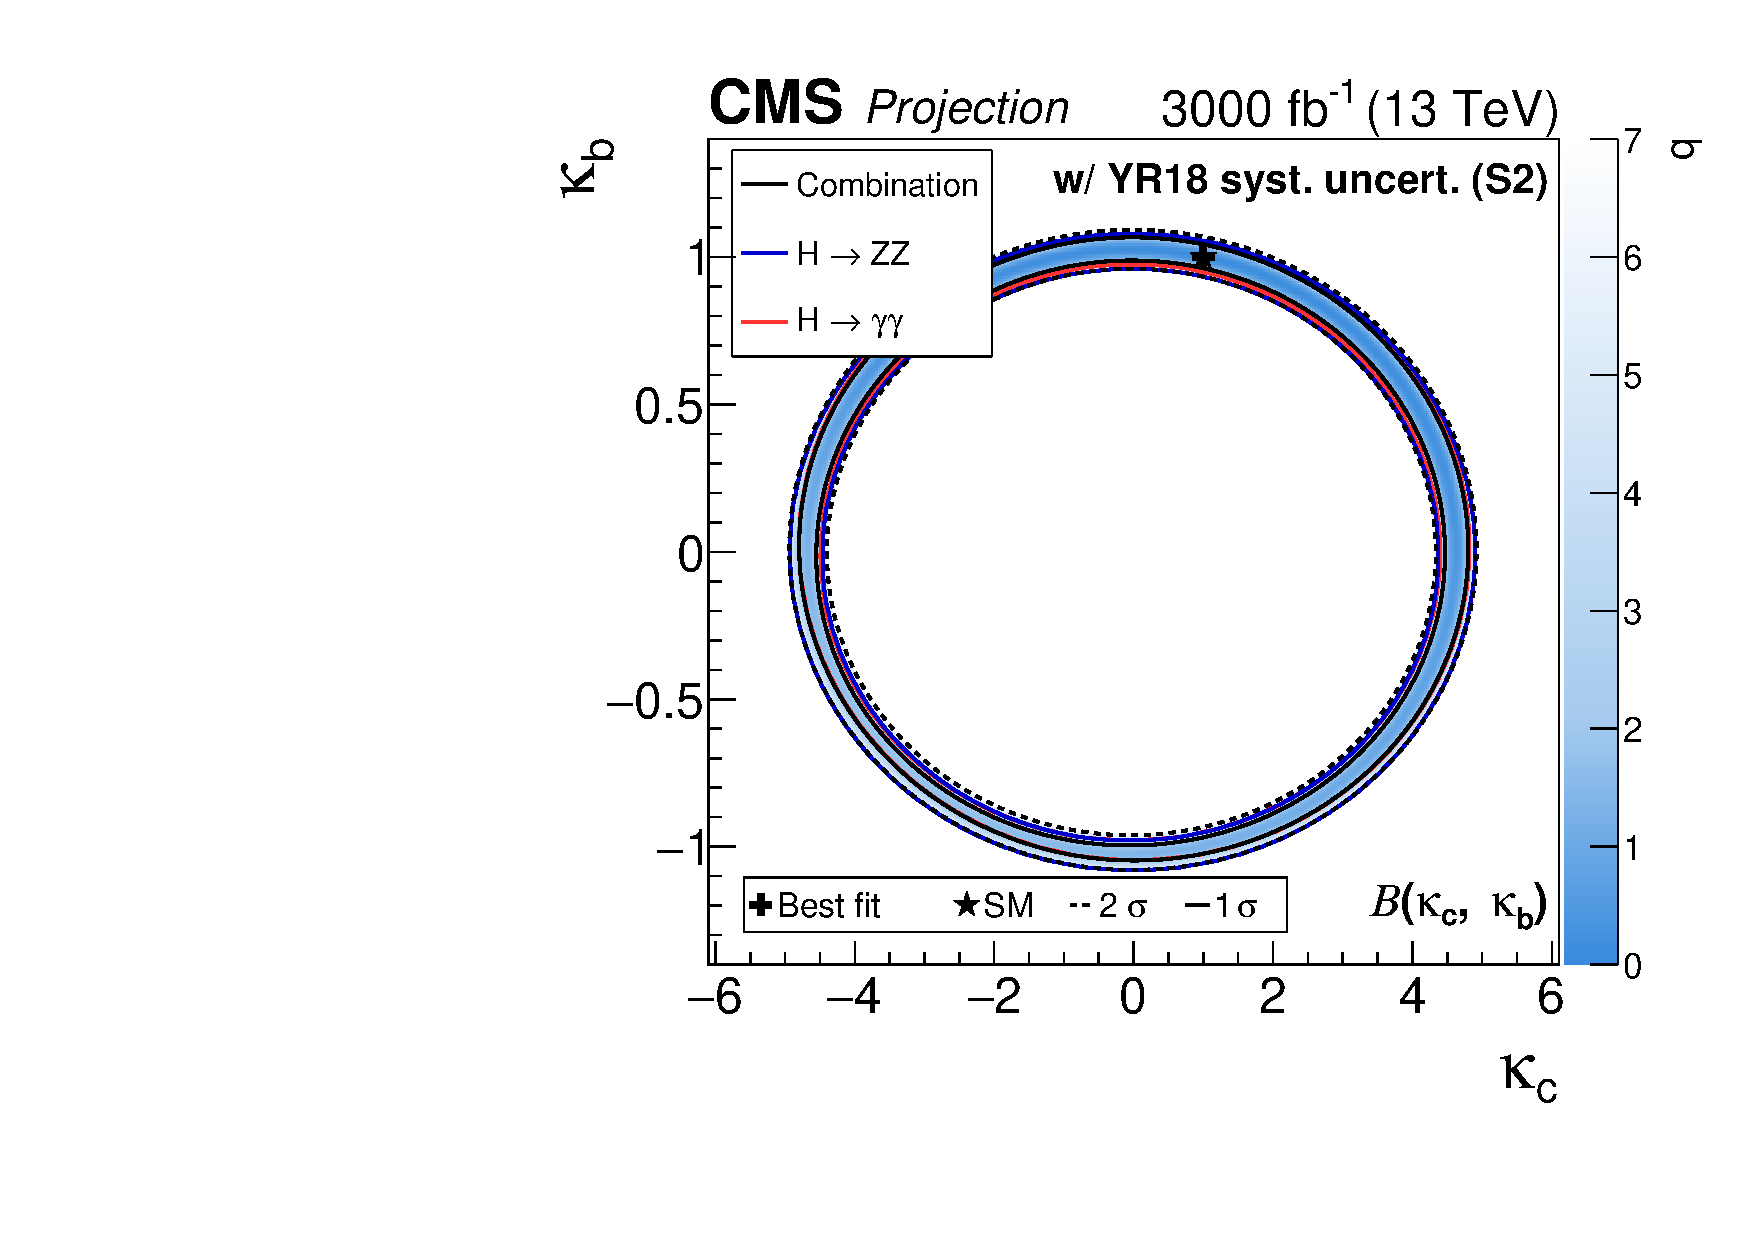
\includegraphics[width=0.49\linewidth]{img/projections/projection_kbkc_plot_couplingdependentBRs_scenario2.pdf}
        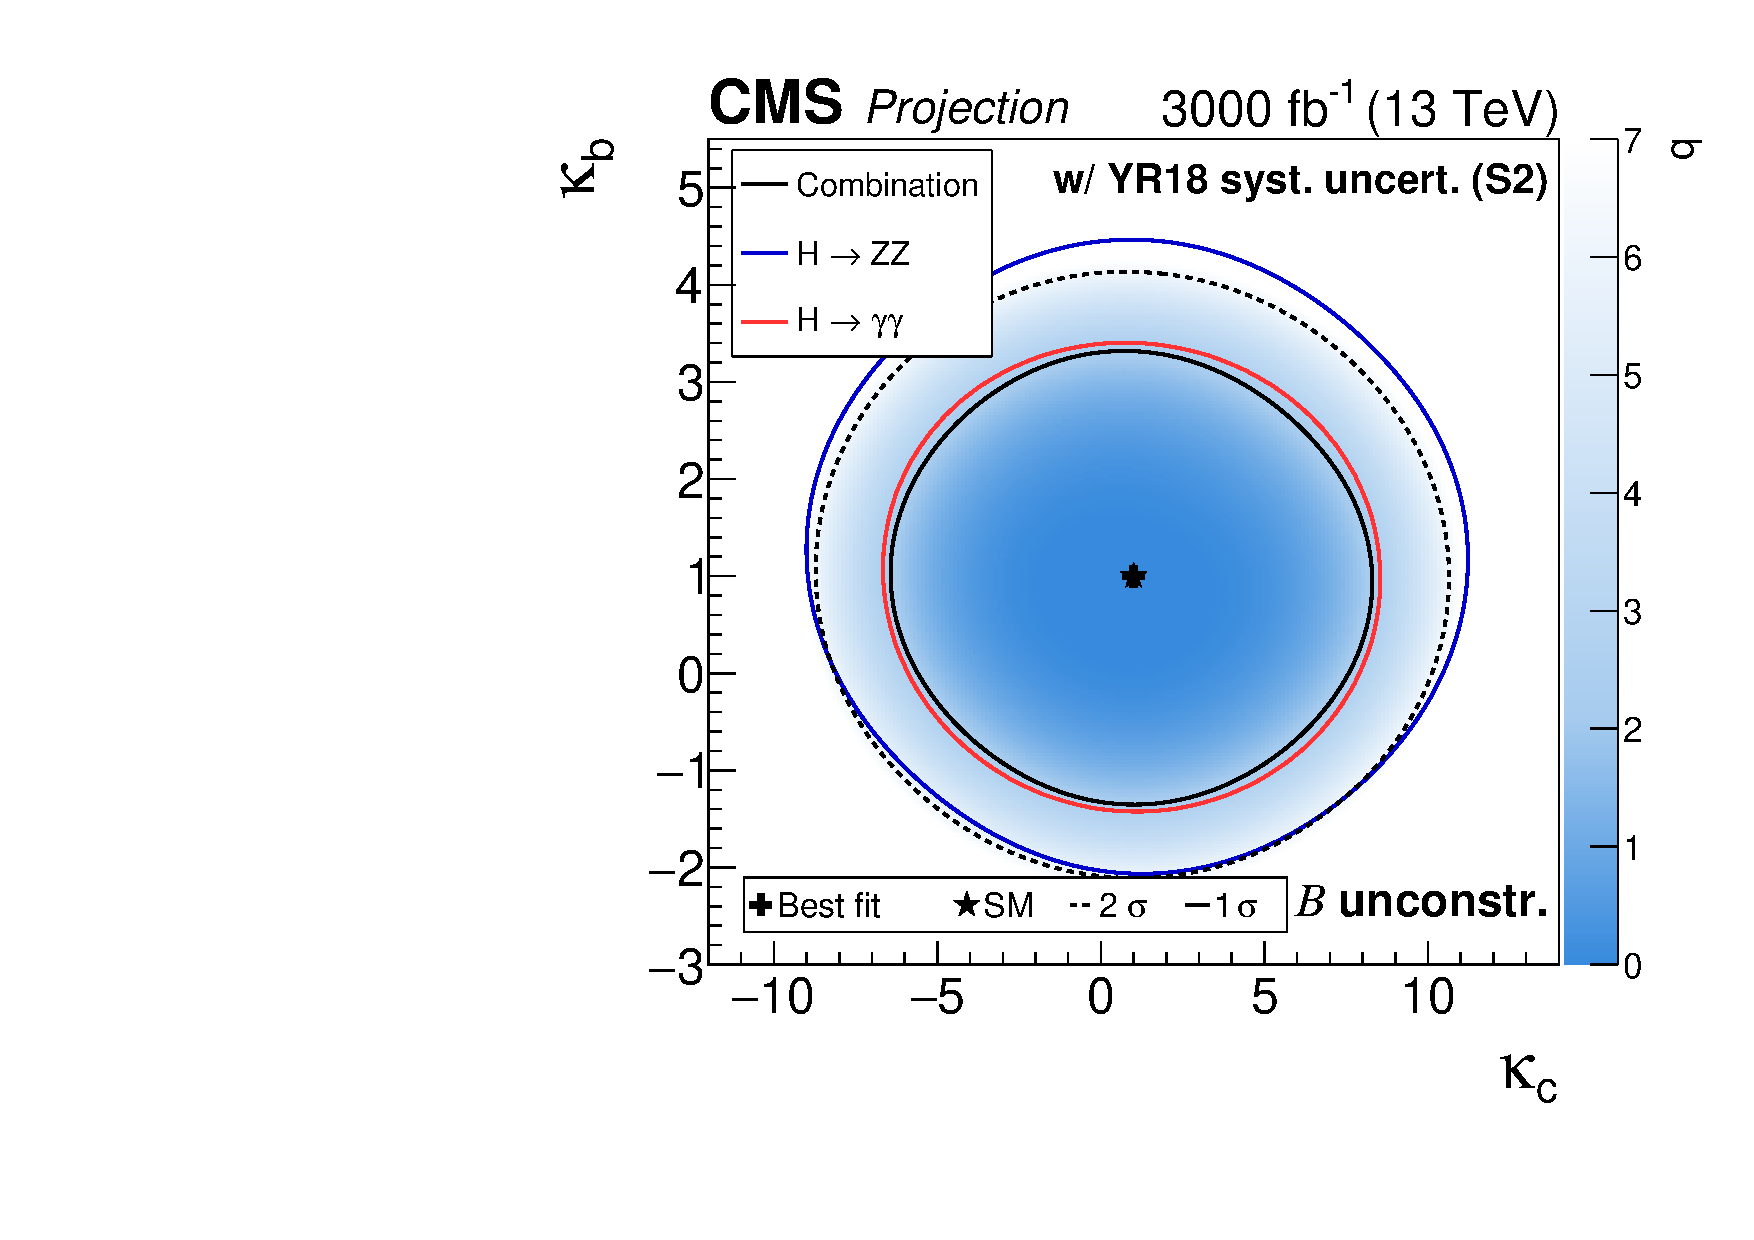
\includegraphics[width=0.49\linewidth]{img/projections/projection_kbkc_plot_floatingBRs_scenario2.pdf}
        }
    % 
    \caption{
        Projected simultaneous fit for $\kappab$ and $\kappac$, assuming a coupling dependence of the branching fractions (left) and the branching fractions implemented as nuisance parameters with no prior constraint (right), under S1 (top) and S2 (bottom).
        % 
        The one standard deviation contour is drawn for the combination ($\hgg$ and $\hzz$), the $\hgg$ channel, and the $\hzz$ channel in black, red, and blue, respectively.
        % 
        For the combination the two standard deviation contour is drawn as a black dashed line, and the shading indicates the negative log-likelihood, with the scale shown on the right hand side of the plots.
        }
    \label{fig:proj_kbkc}
  \end{center}
\end{figure}


\begin{figure}[hbtp]
  \begin{center}
    \ifbool{draftmode}{
        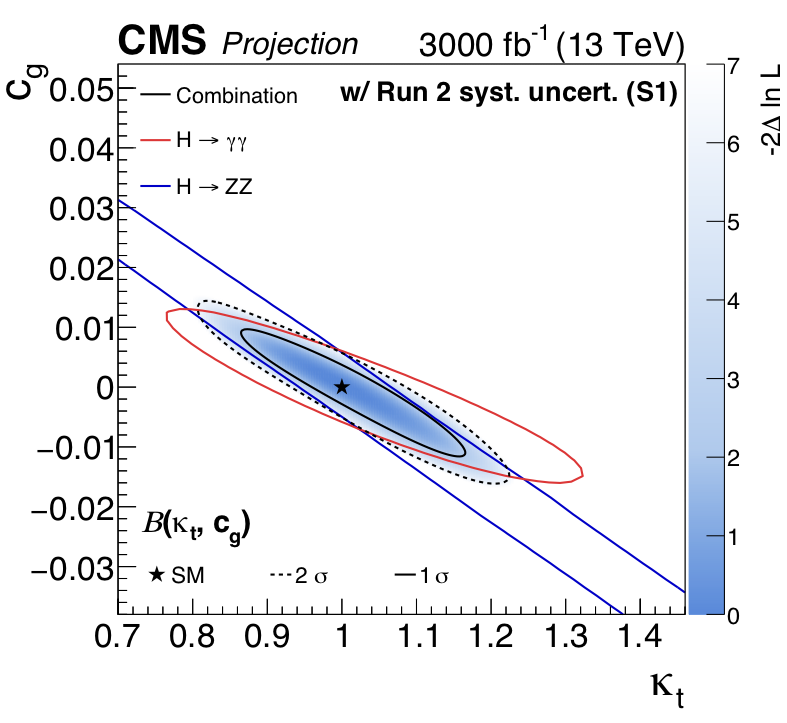
\includegraphics[width=0.49\linewidth]{img/projections/projection_ktcg_plot_couplingdependentBRs.png}
        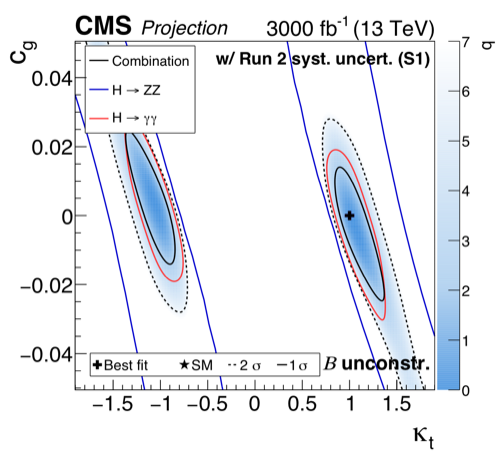
\includegraphics[width=0.49\linewidth]{img/projections/projection_ktcg_plot_floatingBRs.png}
        % 
        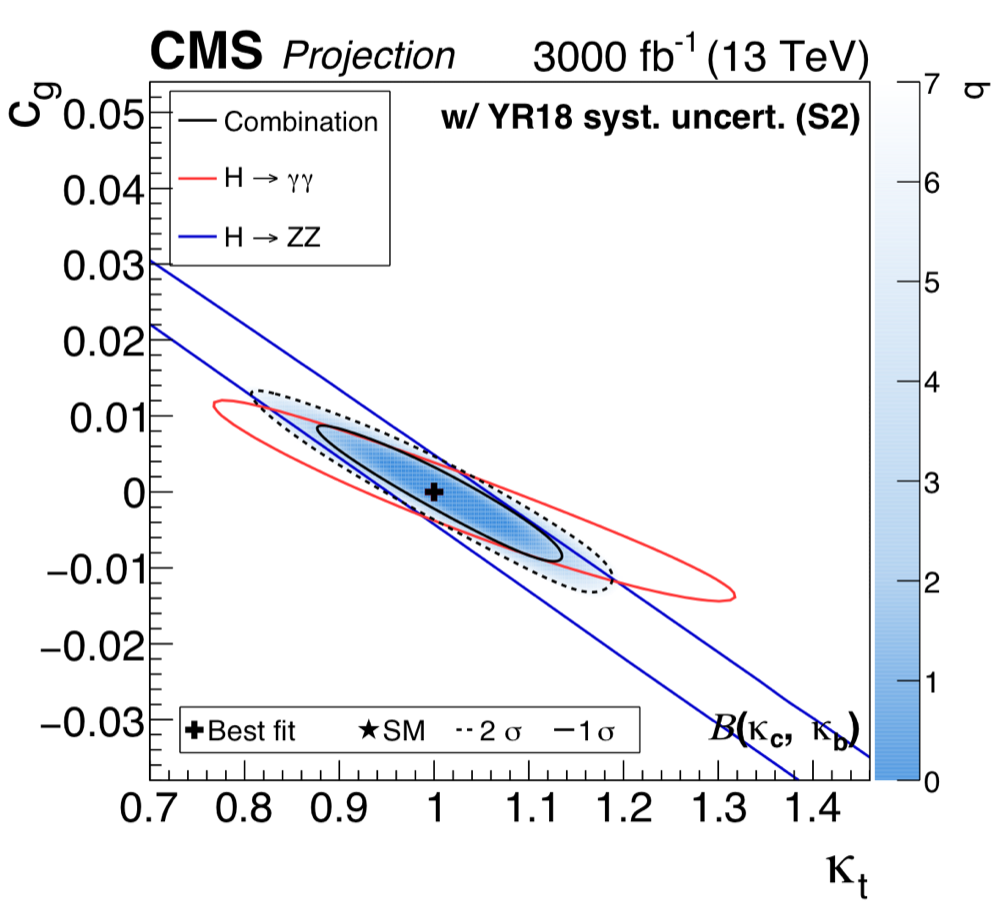
\includegraphics[width=0.49\linewidth]{img/projections/projection_ktcg_plot_couplingdependentBRs_scenario2.png}
        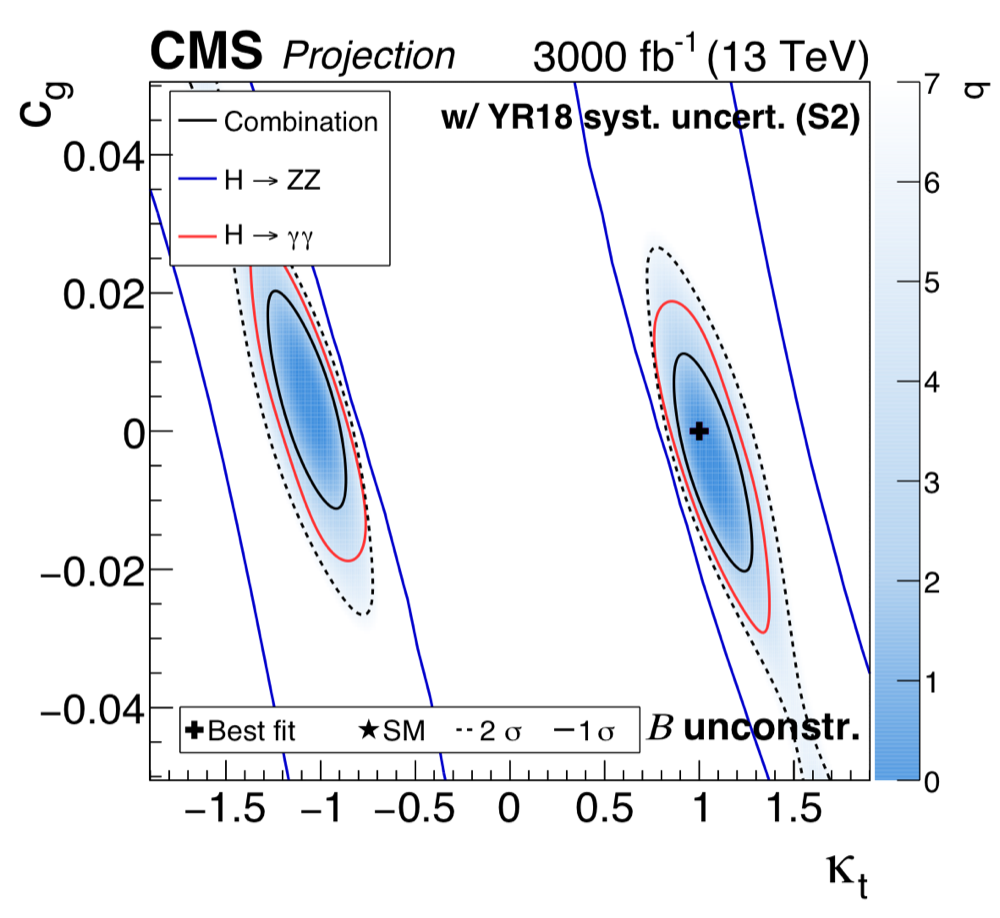
\includegraphics[width=0.49\linewidth]{img/projections/projection_ktcg_plot_floatingBRs_scenario2.png}
        }{
        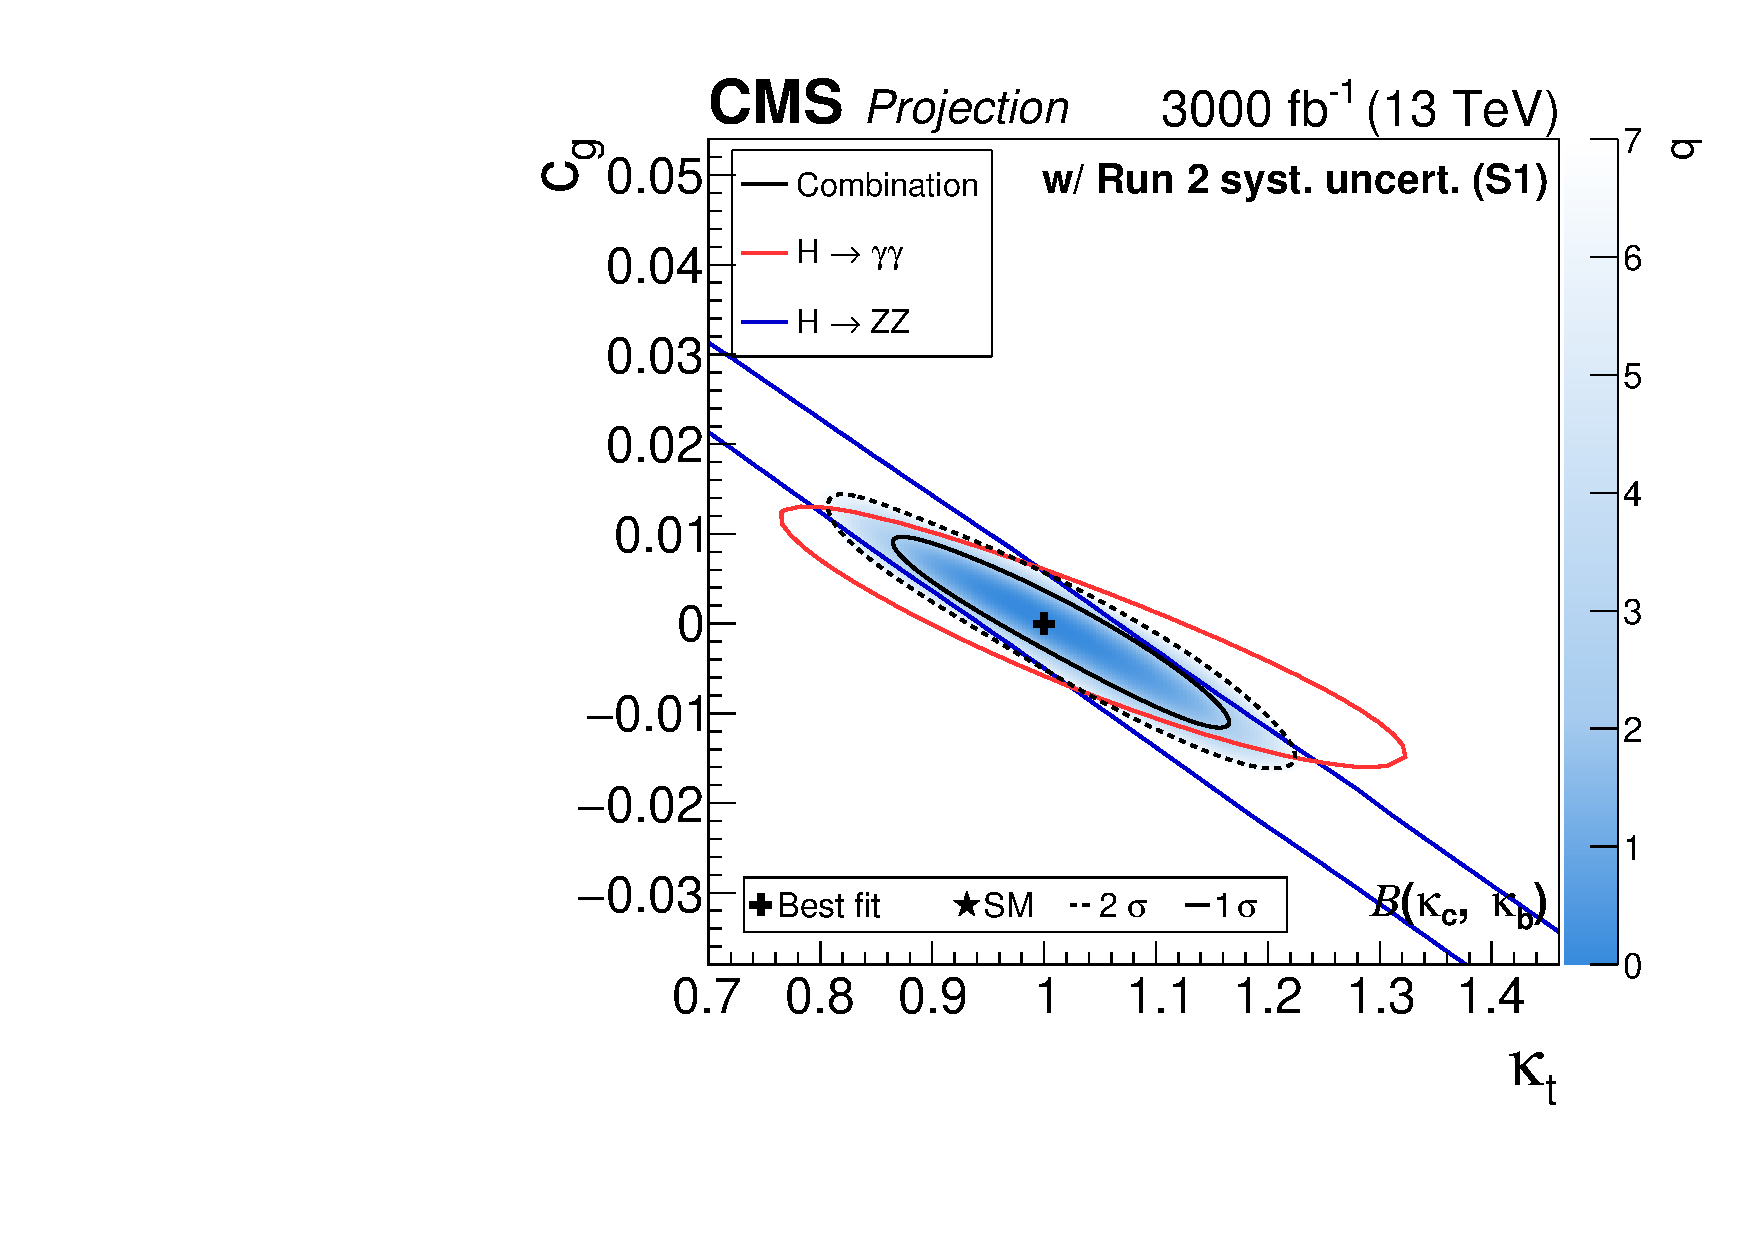
\includegraphics[width=0.49\linewidth]{img/projections/projection_ktcg_plot_couplingdependentBRs.pdf}
        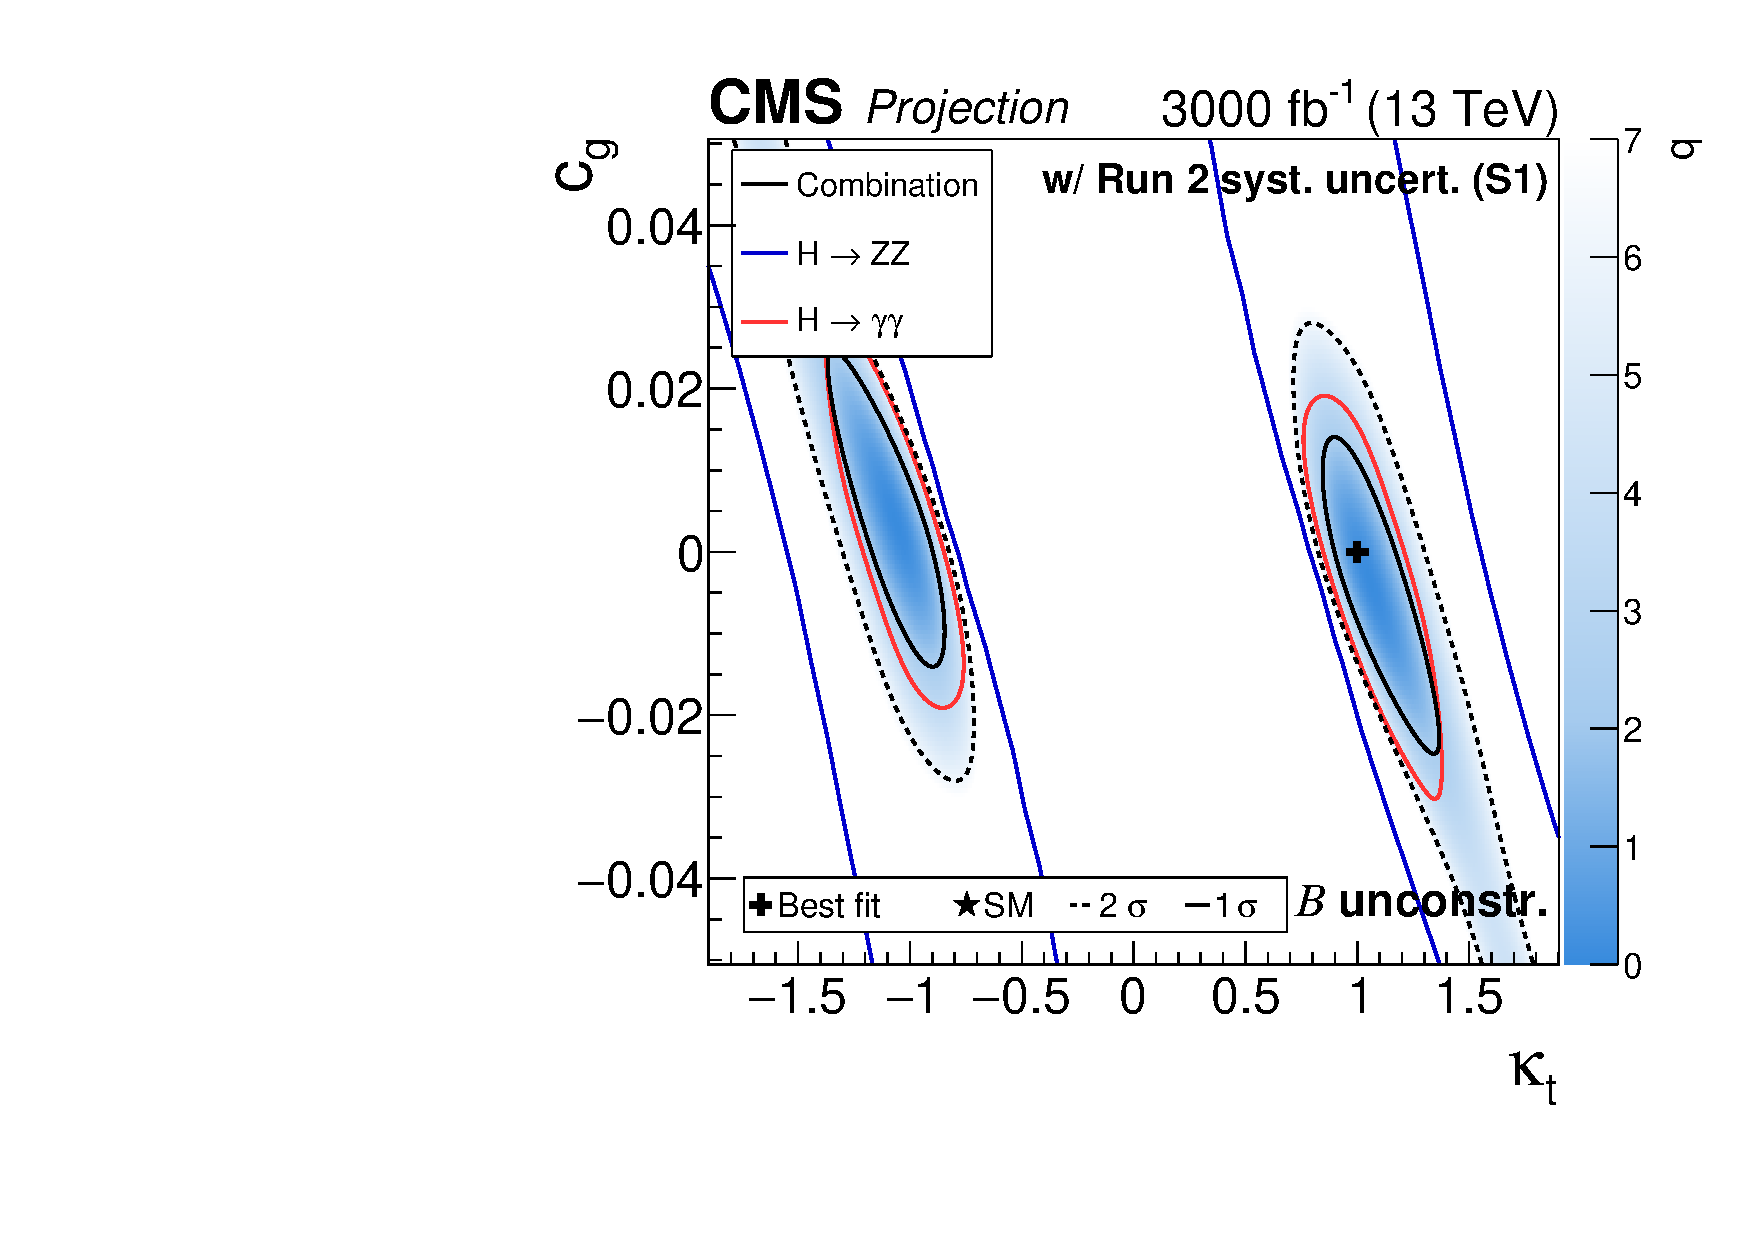
\includegraphics[width=0.49\linewidth]{img/projections/projection_ktcg_plot_floatingBRs.pdf}
        % 
        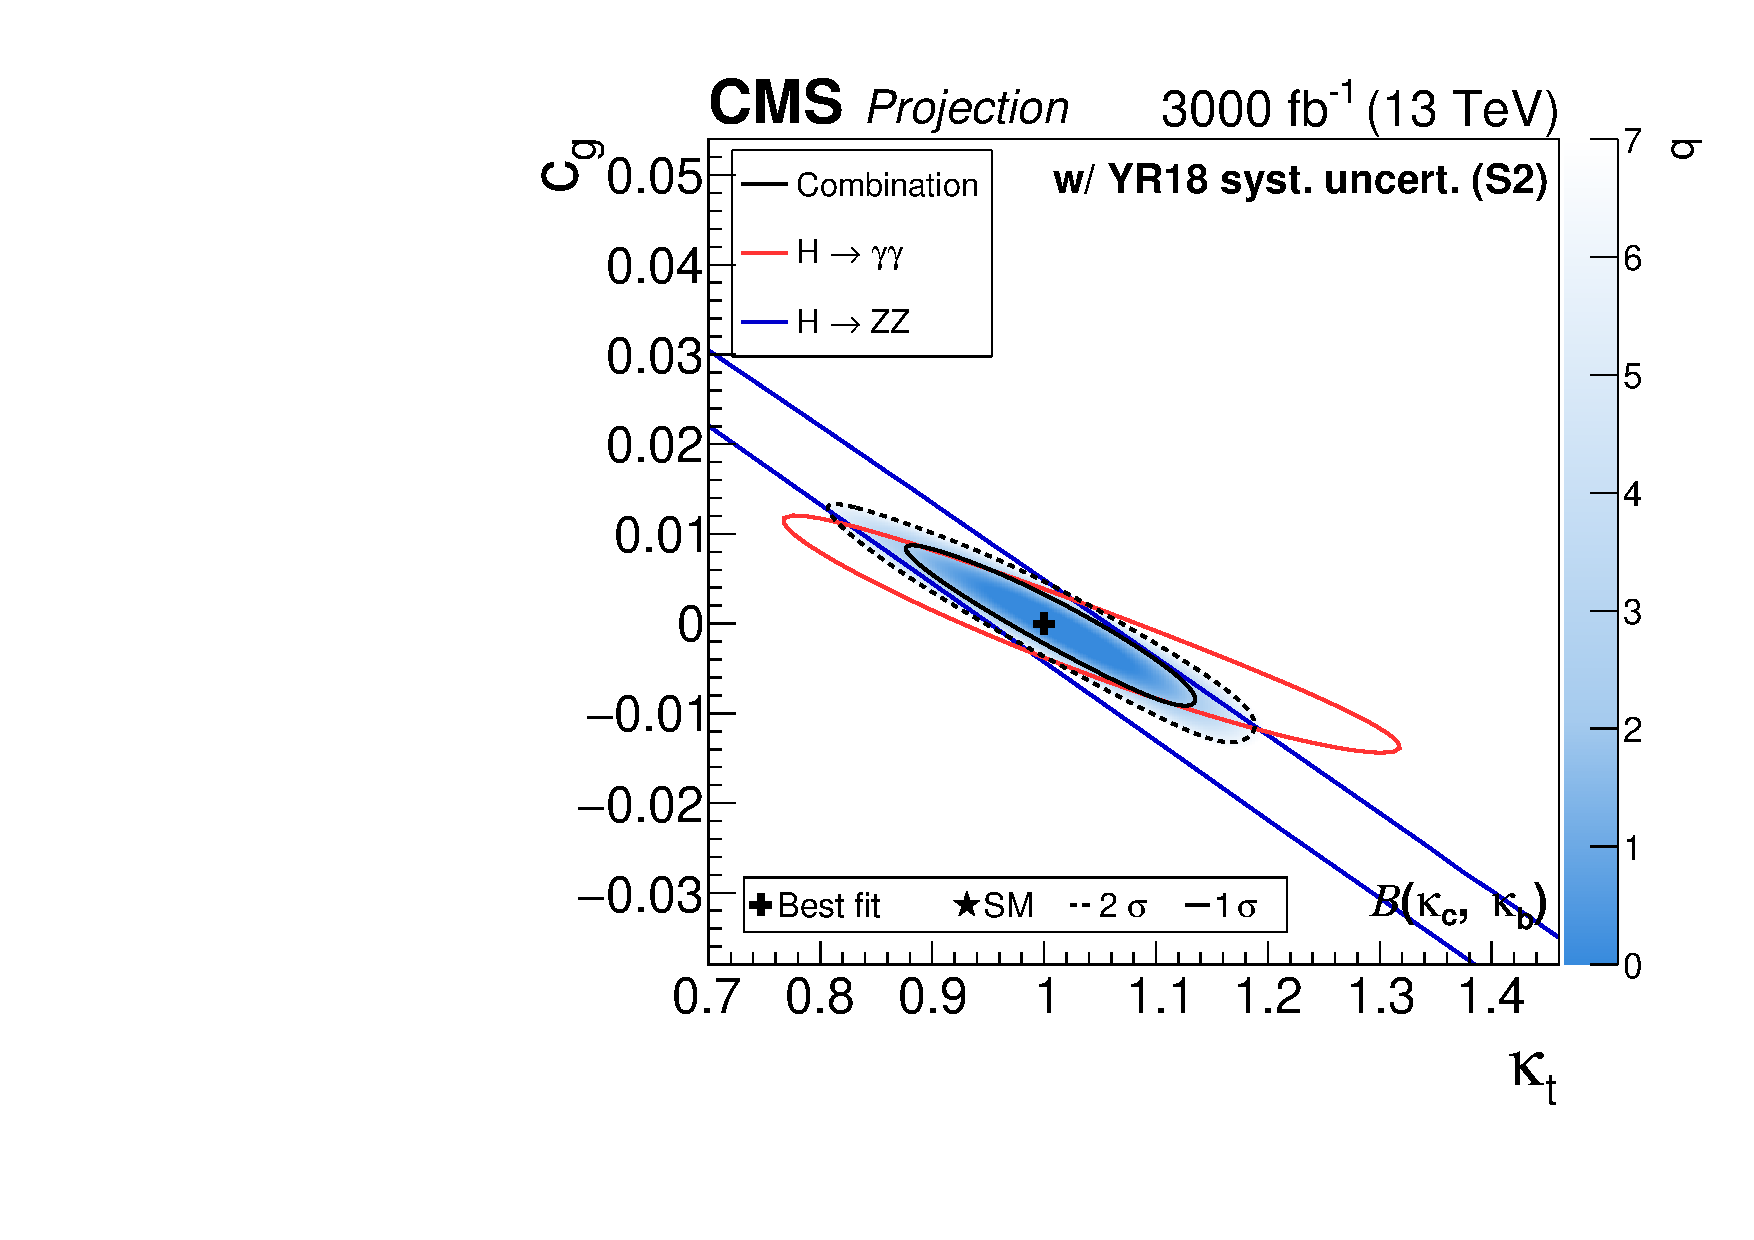
\includegraphics[width=0.49\linewidth]{img/projections/projection_ktcg_plot_couplingdependentBRs_scenario2.pdf}
        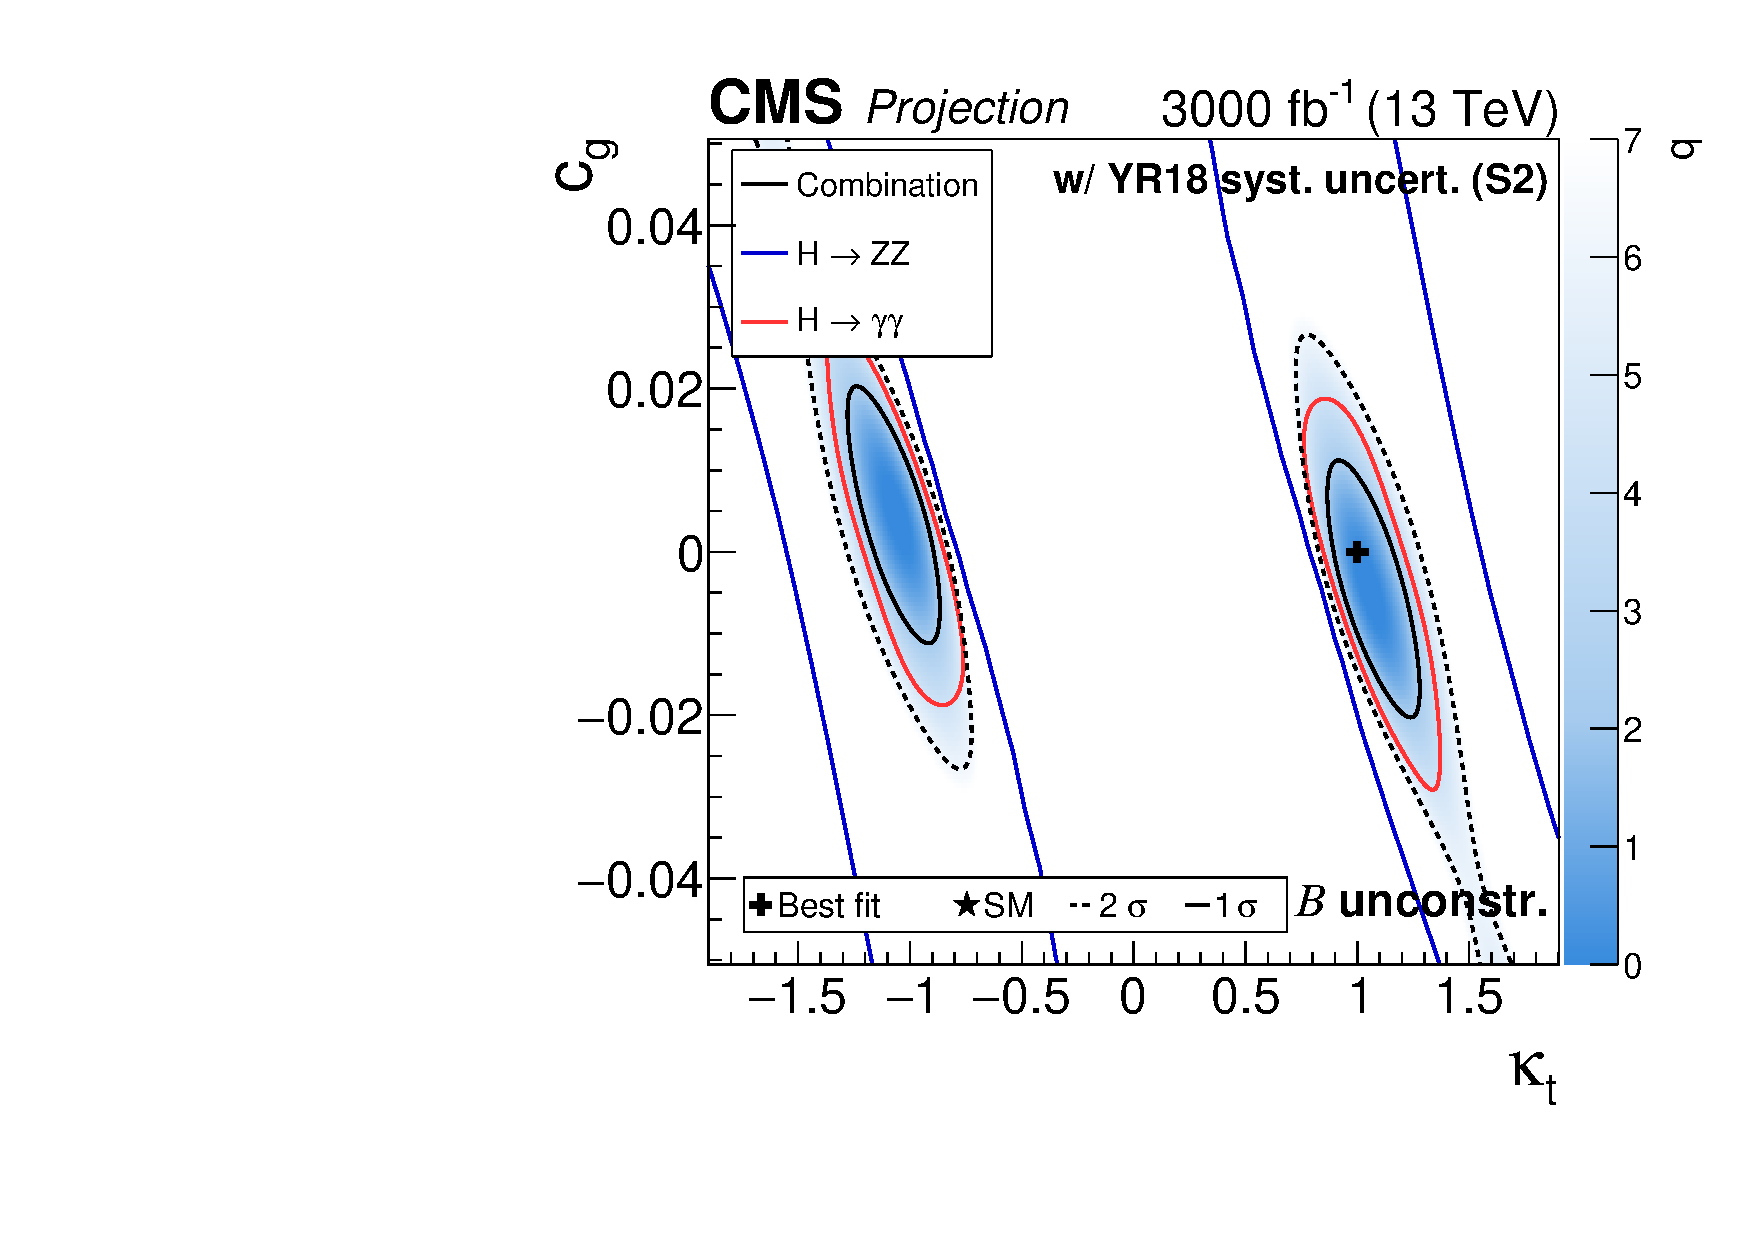
\includegraphics[width=0.49\linewidth]{img/projections/projection_ktcg_plot_floatingBRs_scenario2.pdf}
        }
    % 
    \caption{
        Projected simultaneous fit for $\kappat$ and $\cg$, assuming a coupling dependence of the branching fractions (left) and the branching fractions implemented as nuisance parameters with no prior constraint (right), under S1 (top) and S2 (bottom).
        % 
        The one standard deviation contour is drawn for the combination ($\hgg$, $\hzz$, and $\hbb$), the $\hgg$ channel, and the $\hzz$ channel in black, red, and blue, respectively.
        % 
        For the combination the two standard deviation contour is drawn as a black dashed line, and the shading indicates the negative log-likelihood, with the scale shown on the right hand side of the plots.
        }
    \label{fig:proj_ktcg}
  \end{center}
\end{figure}

